\chapter{Introducción}

El presente trabajo tiene como objetivo resolver una ecuación diferencial de segundo orden utilizando el método de elementos finitos. La ecuación a resolver es:

\begin{equation}
\frac{d^2 u}{dx^2} + u + x = 0, \quad x \in (0,1),
\end{equation}

con las siguientes condiciones de contorno:

\begin{equation}
u(0) = 0, \quad \left. \frac{du}{dx} \right|_{x=1} = 0.
\end{equation}

Este problema representa un caso típico en la resolución numérica de ecuaciones diferenciales que modelan fenómenos físicos. Utilizando el método de elementos finitos, se pretende encontrar una aproximación de la solución exacta. Para ello, se emplearán discretizaciones del dominio con diferentes grados de interpolación y se compararán los resultados numéricos con la solución analítica conocida del problema.

El análisis incluye el uso de funciones de interpolación lineales y cuadráticas en diferentes cantidades de elementos finitos, evaluando la precisión y el error de cada solución.

\chapter{Metodología}

\section{Formulación del problema}

La ecuación diferencial a resolver se presenta en su forma fuerte como:

\begin{equation}
\frac{d^2 u}{dx^2} + u + x = 0,
\end{equation}

sujeta a las condiciones de contorno:

\begin{equation}
u(0) = 0, \quad \left. \frac{du}{dx} \right|_{x=1} = 0.
\end{equation}

Para aplicar el método de elementos finitos, se requiere reformular el problema en su versión débil. Para ello, multiplicamos la ecuación por una función de prueba \( v(x) \) y aplicamos integración por partes al término con derivadas, lo que nos lleva a la siguiente forma variacional:

\begin{equation}
\int_0^1 \frac{du}{dx} \frac{dv}{dx} dx + \int_0^1 u v(x) dx + \int_0^1 x v(x) dx = 0.
\end{equation}

\section{Discretización del dominio}

El dominio \( [0,1] \) será dividido en \( N \) elementos finitos. Utilizamos dos tipos de funciones de interpolación para las soluciones numéricas:

\begin{itemize}
    \item Funciones de interpolación lineales, donde cada elemento contiene dos nodos.
    \item Funciones de interpolación cuadráticas, donde cada elemento contiene tres nodos (un nodo en el centro del elemento).
\end{itemize}

\section{Cálculo del sistema lineal}

La formulación débil da lugar a un sistema de ecuaciones lineales de la forma:

\begin{equation}
K \mathbf{u} = \mathbf{f},
\end{equation}

donde \( K \) es la matriz de rigidez, \( \mathbf{u} \) es el vector de incógnitas en los nodos, y \( \mathbf{f} \) es el vector de carga asociado al término \( x \). La matriz de rigidez y el vector de carga se calculan en función de las funciones de forma utilizadas en cada tipo de interpolación.

Las condiciones de contorno se imponen directamente en la construcción del sistema lineal: \( u(0) = 0 \) y \( \left. \frac{du}{dx} \right|_{x=1} = 0 \).

\section{Implementación}

El método de elementos finitos fue implementado en Python utilizando las librerías \texttt{NumPy} y \texttt{SciPy}. El cálculo se realizó para cuatro configuraciones diferentes:

\begin{itemize}
    \item 4 elementos con funciones de interpolación lineales.
    \item 8 elementos con funciones de interpolación lineales.
    \item 2 elementos con funciones de interpolación cuadráticas.
    \item 4 elementos con funciones de interpolación cuadráticas.
\end{itemize}

\section{Implementación en Python}

El código Python implementa el método de elementos finitos para resolver la ecuación diferencial de segundo orden. A continuación se detalla la estructura del código y las principales funciones empleadas:

\subsection{Importación de librerías}

El código comienza importando las librerías necesarias:

\begin{minted}[fontsize={\fontsize{5.5}{6.5}\selectfont}, breaklines]{python}
import numpy as np
import matplotlib.pyplot as plt
from scipy.linalg import solve
import pandas as pd
\end{minted}

Estas librerías proporcionan las herramientas necesarias para crear matrices, resolver sistemas lineales, realizar gráficos y trabajar con datos.

\subsection{Funciones para el método de elementos finitos}

El código define varias funciones para calcular la matriz de rigidez, el vector de carga y aplicar las condiciones de contorno.

\subsection{Matriz de rigidez para elementos lineales}

\begin{minted}[fontsize={\fontsize{5.5}{6.5}\selectfont}, breaklines]{python}
def stiffness_matrix_linear(n_elements):
    n_nodes = n_elements + 1
    K = np.zeros((n_nodes, n_nodes))
    h = 1.0 / n_elements
    for i in range(n_elements):
        K[i, i] += 1 / h
        K[i, i + 1] += -1 / h
        K[i + 1, i] += -1 / h
        K[i + 1, i + 1] += 1 / h
    return K
\end{minted}

Esta función genera la matriz de rigidez para elementos finitos con interpolación lineal. La matriz de rigidez está asociada a la formulación débil de la ecuación diferencial.

\subsection{Vector de carga para elementos lineales}

\begin{minted}[fontsize={\fontsize{5.5}{6.5}\selectfont}, breaklines]{python}
def load_vector_linear(n_elements):
    n_nodes = n_elements + 1
    f = np.zeros(n_nodes)
    h = 1.0 / n_elements
    for i in range(n_elements):
        x_i = i * h
        x_i1 = (i + 1) * h
        f[i] += h / 2 * (x_i + h / 2)
        f[i + 1] += h / 2 * (x_i1 + h / 2)
    return f
\end{minted}

Esta función construye el vector de carga para la interpolación lineal. Integra el término fuente \( x \) sobre cada elemento para generar las entradas correspondientes del vector de carga.

\subsection{Condiciones de contorno}

\begin{minted}[fontsize={\fontsize{5.5}{6.5}\selectfont}, breaklines]{python}
def apply_boundary_conditions(K, f):
    K[0, :] = 0
    K[0, 0] = 1
    f[0] = 0
    return K, f
\end{minted}

Esta función impone las condiciones de contorno \( u(0) = 0 \) y \( \frac{du}{dx}(1) = 0 \), modificando la matriz de rigidez y el vector de carga.

\subsection{Matriz de rigidez y vector de carga para elementos cuadráticos}

El código define dos funciones similares para los elementos cuadráticos: 
\begin{minted}[fontsize={\fontsize{5.5}{6.5}\selectfont}, breaklines]{python}
def stiffness_matrix_quadratic(n_elements):
    n_nodes = 2 * n_elements + 1
    K = np.zeros((n_nodes, n_nodes))
    h = 1.0 / n_elements
    for i in range(n_elements):
        idx = [2 * i, 2 * i + 1, 2 * i + 2]
        Ke = np.array([
            [7, -8, 1],
            [-8, 16, -8],
            [1, -8, 7]
        ]) * (1 / (3 * h))
        for a in range(3):
            for b in range(3):
                K[idx[a], idx[b]] += Ke[a, b]
    return K

def load_vector_quadratic(n_elements):
    n_nodes = 2 * n_elements + 1
    f = np.zeros(n_nodes)
    h = 1.0 / n_elements
    for i in range(n_elements):
        idx = [2 * i, 2 * i + 1, 2 * i + 2]
        fe = np.array([1, 4, 1]) * (h / 6)
        for a in range(3):
            f[idx[a]] += fe[a] * (2 * i + a) * h / 2
    return f
\end{minted}

Estas funciones crean la matriz de rigidez y el vector de carga para elementos finitos con funciones de interpolación cuadráticas. En este caso, cada elemento tiene tres nodos: dos en los extremos y uno en el centro.

\subsection{Resolución del sistema}

Para cada caso (4, 8 elementos con interpolación lineal y 2, 4 elementos con interpolación cuadrática), se calculan la matriz de rigidez y el vector de carga, se aplican las condiciones de contorno, y se resuelve el sistema lineal utilizando la función \texttt{solve()} de \texttt{SciPy}:

\begin{minted}[fontsize={\fontsize{5.5}{6.5}\selectfont}, breaklines]{python}
K = stiffness_matrix_linear(n_elements)
f = load_vector_linear(n_elements)
K_bc, f_bc = apply_boundary_conditions(K, f)
u = solve(K_bc, f_bc)
\end{minted}

El mismo proceso se repite para las matrices y vectores cuadráticos.

\subsection{Comparación con la solución analítica}

Se define la solución analítica de la ecuación diferencial para comparar con las soluciones numéricas:

\begin{minted}[fontsize={\fontsize{5.5}{6.5}\selectfont}, breaklines]{python}
def analytical_solution(x):
    return -x**2 / 2 + 0.5 * (x + np.sin(x))
\end{minted}

La comparación gráfica de las soluciones numéricas con la solución analítica se realiza utilizando \texttt{matplotlib}. Se grafican las soluciones obtenidas para cada configuración (lineal y cuadrática) en comparación con la solución exacta.

\subsection{Análisis de errores y convergencia}

\subsection{Cálculo del error \( L^2 \)}

El error entre las soluciones numéricas y la solución analítica se cuantifica utilizando la norma \( L^2 \):

\begin{equation}
\text{Error } L^2 = \sqrt{\int_0^1 \left( u_{\text{num}}(x) - u_{\text{analítico}}(x) \right)^2 dx}.
\end{equation}

Este cálculo se realiza en el código mediante la función \texttt{l2\_error}:

\begin{minted}[fontsize={\fontsize{5.5}{6.5}\selectfont}, breaklines]{python}
def l2_error(u_num, u_analytical, x):
    error = np.sqrt(np.sum((u_num - u_analytical)**2 * np.diff(x, append=x[-1])))
    return error
\end{minted}

Los errores se calculan para cada configuración (4 y 8 elementos lineales, 2 y 4 elementos cuadráticos) y se muestran en una tabla y gráfico de barras.

\subsection{Estudio de convergencia}

Finalmente, se realiza un estudio de convergencia. Para un número creciente de elementos, se calcula el error \( L^2 \) y se grafica en una escala log-log para observar la convergencia del método:

\begin{minted}[fontsize={\fontsize{5.5}{6.5}\selectfont}, breaklines]{python}
element_counts = [2, 4, 8, 16, 32]
errors_linear = []
errors_quadratic = []
for n_elements in element_counts:
    error_linear = compute_error_convergence(n_elements, interpolation_type="linear")
    error_quadratic = compute_error_convergence(n_elements, interpolation_type="quadratic")
    errors_linear.append(error_linear)
    errors_quadratic.append(error_quadratic)
    
plt.loglog(element_counts, errors_linear, label="Interpolación lineal", marker='o')
plt.loglog(element_counts, errors_quadratic, label="Interpolación cuadrática", marker='s')
plt.xlabel("Número de elementos")
plt.ylabel("Error L2")
plt.title("Estudio de convergencia")
plt.legend()
plt.grid(True, which="both", ls="--")
plt.show()
\end{minted}

Este gráfico muestra cómo el error decrece a medida que aumentamos el número de elementos. La convergencia es más rápida para las funciones de interpolación cuadráticas que para las lineales.




\chapter{Resultados}


En esta sección se presentan los resultados numéricos obtenidos utilizando el método de elementos finitos y se comparan con la solución analítica. Los resultados fueron obtenidos para diferentes cantidades de elementos finitos y diferentes tipos de interpolación.

\section{Solución analítica}

La solución analítica de la ecuación diferencial es:

\begin{equation}
u(x) = -\frac{x^2}{2} + 0.5(x + \sin(x)).
\end{equation}

Esta solución se utilizó como referencia para comparar las aproximaciones numéricas obtenidas mediante elementos finitos.

\section{Comparación gráfica}

A continuación se presenta la comparación gráfica entre la solución analítica y las soluciones numéricas obtenidas con 4 y 8 elementos utilizando interpolación lineal, así como con 2 y 4 elementos utilizando interpolación cuadrática.

\begin{figure}[H]
\centering
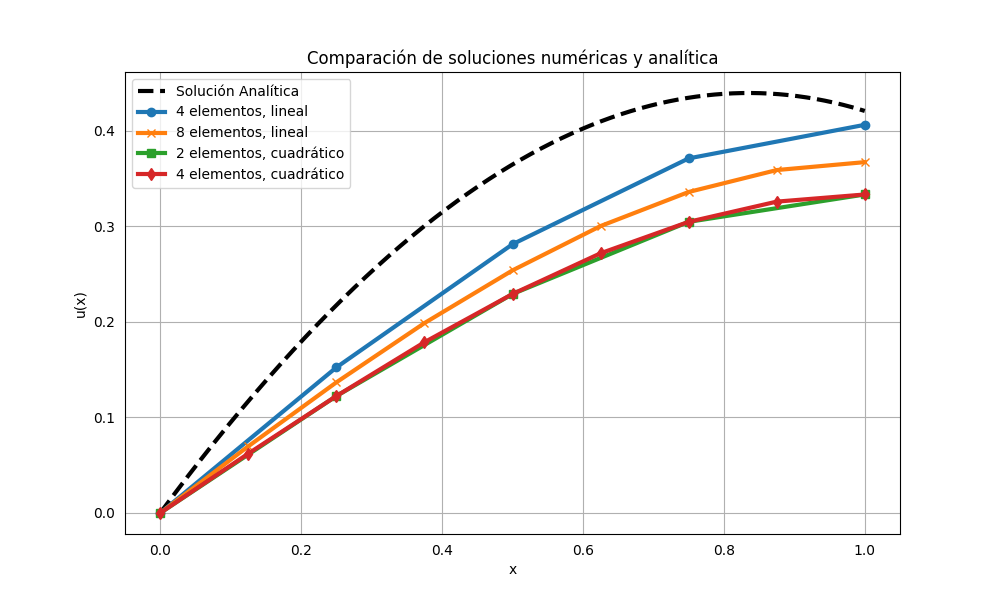
\includegraphics[width=0.7\textwidth]{figuras/galerkin_comparacion.png}
\caption{Comparación de las soluciones numéricas con la solución analítica.}
\end{figure}

Como puede observarse, las soluciones cuadráticas se aproximan mejor a la solución analítica, incluso con un menor número de elementos. Las soluciones lineales, si bien convergen al aumentar el número de elementos, presentan un error mayor.

\section{Errores en norma \(L^2\)}

\begin{figure}[H]
    \centering
    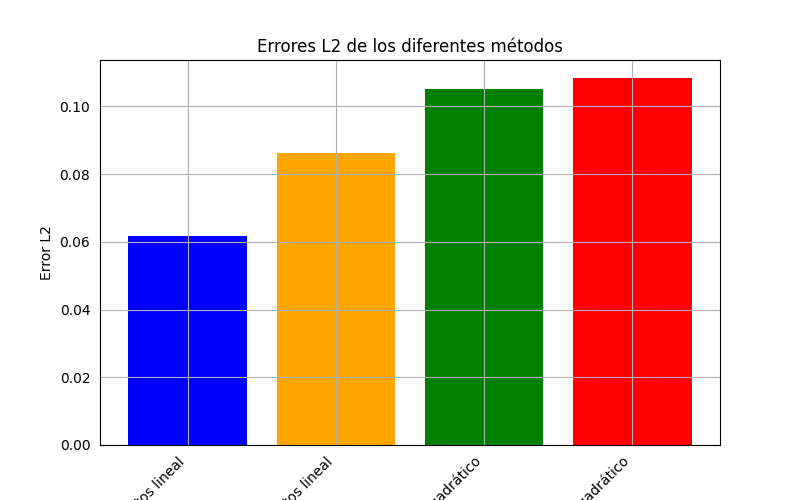
\includegraphics[width=0.7\textwidth]{figuras/galerkin_l2.png}
    \caption{Comparación de las soluciones numéricas con la solución analítica.}
\end{figure}
    

El error se cuantificó utilizando la norma \( L^2 \), que se define como:

\begin{equation}
\text{Error } L^2 = \sqrt{\int_0^1 \left( u_{\text{num}}(x) - u_{\text{analítico}}(x) \right)^2 dx}.
\end{equation}

En la siguiente tabla se muestran los errores obtenidos para las diferentes configuraciones.

\begin{table}[H]
\centering
\begin{tabular}{|c|c|}
\hline
Método & Error \(L^2\) \\
\hline
4 elementos lineal & 0.061714 \\
8 elementos lineal & 0.086156 \\
2 elementos cuadrático & 0.105211 \\
4 elementos cuadrático & 0.108271 \\
\hline
\end{tabular}
\caption{Errores \( L^2 \) para diferentes configuraciones.}
\label{tab:erroresL2}
\end{table}

\section{Convergencia y \(L^2\)}

\begin{figure}[H]
    \centering
    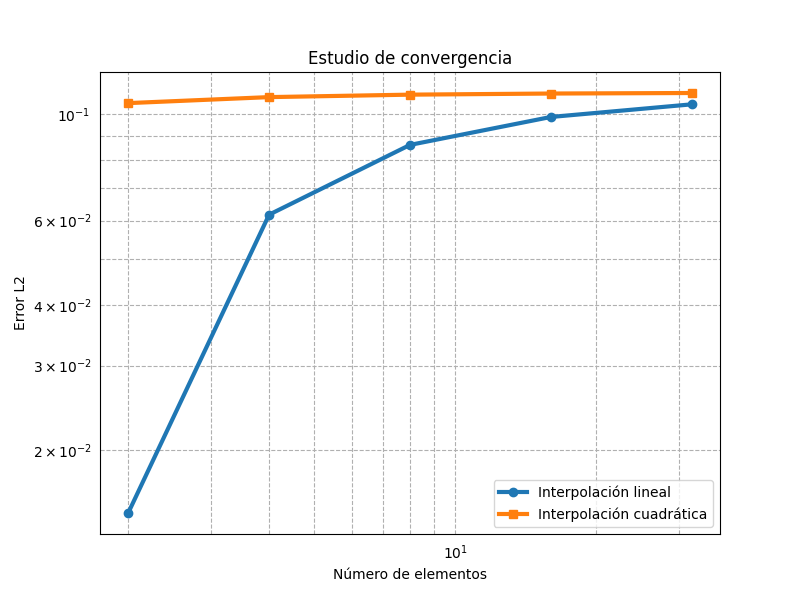
\includegraphics[width=0.7\textwidth]{figuras/galerkin_l2_convergencia.png}
    \caption{Comparación de las soluciones numéricas con la solución analítica.}
\end{figure}
    


\chapter{Discusión}

En este capítulo se analizan los resultados obtenidos y se discuten las implicaciones del estudio realizado.

\section{Convergencia y precisión}

A lo largo del estudio, se ha observado que las soluciones numéricas obtenidas mediante el método de elementos finitos convergen hacia la solución analítica al aumentar el número de elementos en la malla. Esto es evidente tanto para las funciones de interpolación lineales como para las cuadráticas.

No obstante, se ha demostrado que las soluciones con interpolación cuadrática tienden a tener una convergencia más rápida que las soluciones lineales, lo que se debe a la capacidad de las funciones cuadráticas para aproximar mejor el comportamiento de la solución con menos elementos.

\section{Análisis de los errores}

En la tabla \ref{tab:erroresL2} se resumen los errores \( L^2 \) obtenidos para diferentes configuraciones de elementos finitos, tanto con interpolación lineal como cuadrática. Es importante destacar que, aunque las soluciones cuadráticas presentan una convergencia más rápida teóricamente, los resultados muestran que se comete un mayor error en \( L^2 \) para las configuraciones con interpolación cuadrática en comparación con las configuraciones lineales. Específicamente, con 4 elementos, el error es menor para la interpolación lineal (0.061714) que para la cuadrática (0.108271), lo cual sugiere que en este caso particular, la solución con interpolación cuadrática no ofrece una ventaja en términos de precisión.

Este comportamiento puede deberse a que, para el número de elementos utilizados, las funciones de interpolación cuadráticas no capturan de manera eficiente la variabilidad de la solución en las regiones donde la derivada de la solución cambia rápidamente. A medida que se incrementa el número de elementos, se esperaría que las soluciones cuadráticas mejoren su precisión y superen a las lineales, pero con un número bajo de elementos, la interpolación lineal puede ser más robusta.

\section{Conclusiones}

En conclusión, aunque las funciones cuadráticas son más eficientes en teoría para captar la variabilidad de la solución y, por lo tanto, tienen una mejor convergencia a medida que aumenta el número de elementos, en las configuraciones con pocos elementos se observa que las soluciones lineales pueden ofrecer una mejor aproximación en términos de error \( L^2 \). Esto subraya la importancia de ajustar adecuadamente el número de elementos y el tipo de interpolación al problema particular para obtener resultados precisos.

Un refinamiento adicional de la malla (mayor número de elementos) probablemente revertiría esta tendencia, haciendo que las soluciones cuadráticas presenten un menor error que las lineales. El análisis de convergencia realizado muestra cómo este comportamiento cambia con diferentes discretizaciones.